\chapter{Usage Guide}
\label{chap:usage_guide}


\section{Mono-procedures}


\subsection{Authenticated}

\subsubsection{Log in to the system}
\vspace{0.5cm}
\hrule
\begin{lyxlist}{PC1}
\small{
\item [\textbf{Procedure:}] Login
\item [\textbf{Scope:}] Crisis Management System (\emph{CMS})
\item [\textbf{Primary Actor}:] Authenticated Kuzma
\item [\textbf{Goal:}] To login to the system
\item [\textbf{Level}:] User-goal level
\item [\textbf{Main~Success~Scenario}]:\\
1. \emph{Kuzma} enters his login 'icrashadmin' and password 'qwerty'. \\
2. \emph{Kuzma} click button `Logon`.\\
3. \emph{CMS} checks that login and password correct.\\
4. \emph{CMS} informs \emph{Kuzma} that he is authenticated.\\
\item [\textbf{Extensions}]:\\
3.a \emph{CMS} detects that login or password incorrect.\\
\hspace*{0.5cm} 1.a.1 \emph{CMS} shows the warning 'Incorrect data'\\ 
\hspace*{0.5cm} \textbf{procedure continues at step 1}\\
3.b \emph{Kuzma} detects that login or password was enetered incorrectly three
times\\
\hspace*{0.5cm} 3.b.1 \emph{CMS} shows captcha test.\\ 
\hspace*{0.5cm} 3.b.2 \emph{Kuzma} types characters '504375' from the image.\\ 
\hspace*{0.5cm} 3.b.3.1 \emph{CMS} checks that answer to captcha test is
correct.\\
\hspace*{0.5cm} \textbf{procedure continues at step 1} \\
\hspace*{0.5cm} 3.b.3.2 \emph{CMS} detects that answer to captcha test was
enetered incorrectly.\\
\hspace*{0.5cm} \textbf{procedure continues at step 3.b.1}
}
\end{lyxlist}
\hrule
\vspace{0.5cm}

\begin{figure}[h]
    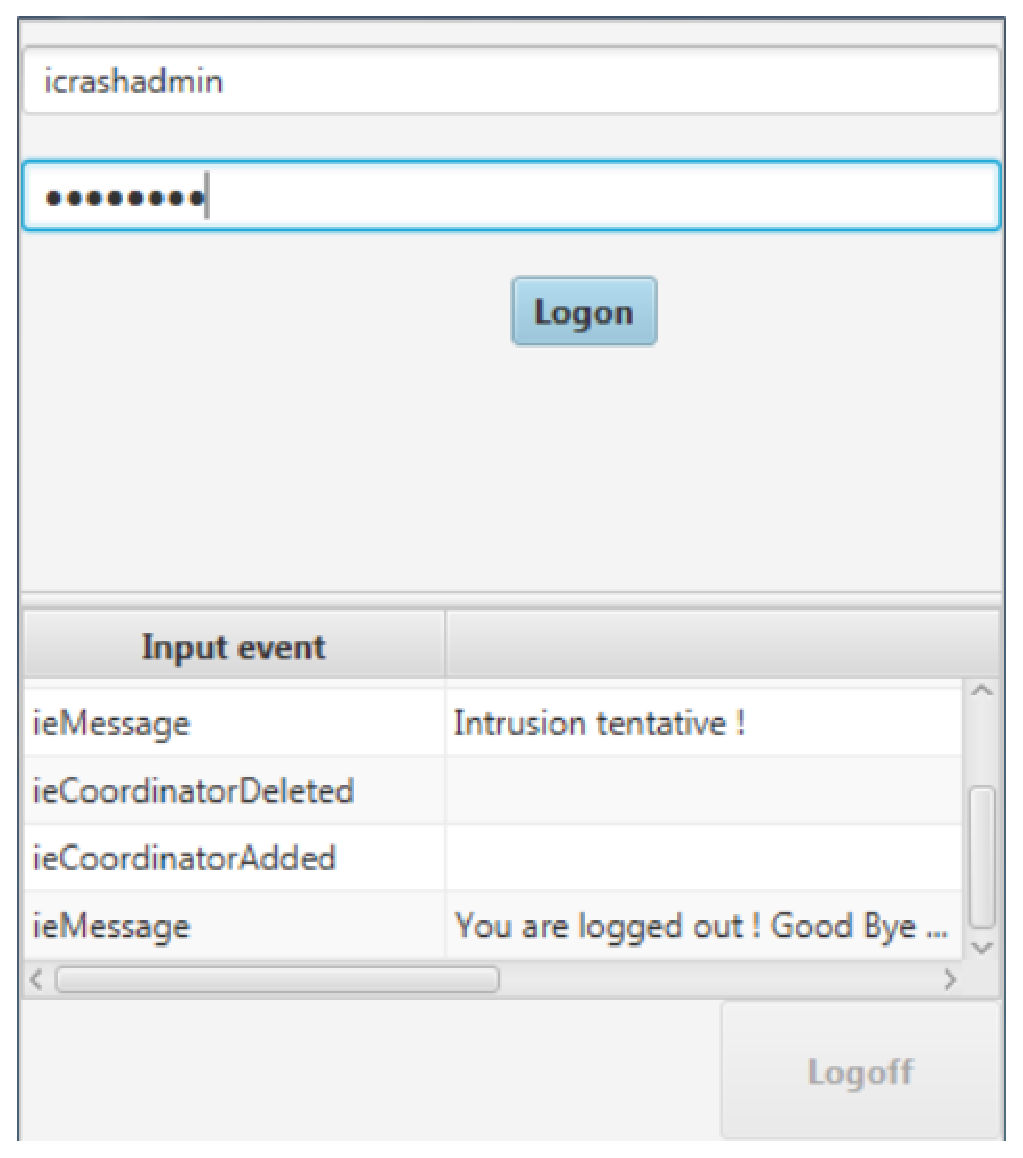
\includegraphics[scale=0.75]{login2.eps}
	\caption{Login in the system}
\end{figure}

\begin{figure}[h]
    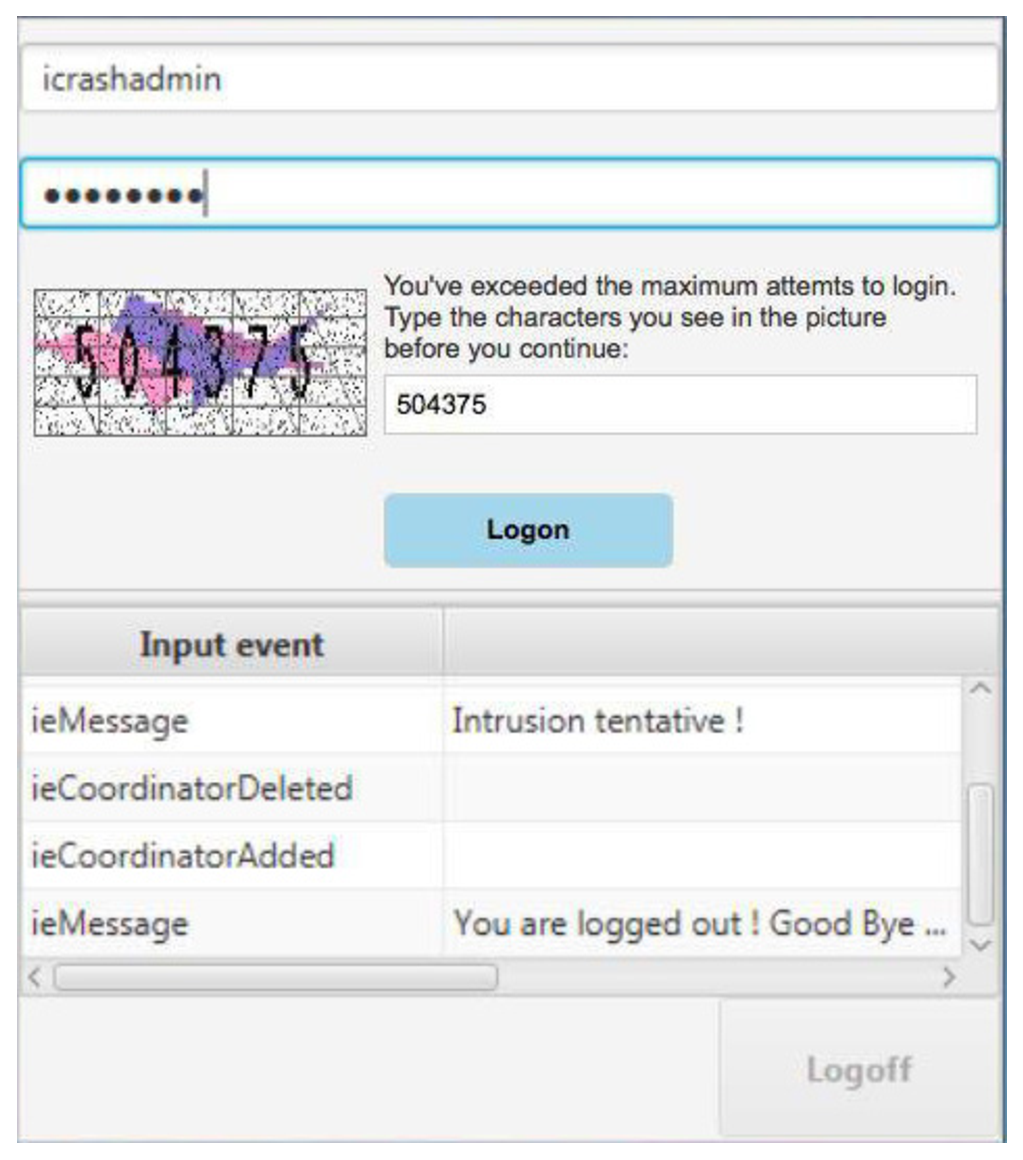
\includegraphics[scale=0.75]{login.eps}
	\caption{Captcha test}
\end{figure}

\subsubsection{Log out from the system}
\vspace{0.5cm}
\hrule
\begin{lyxlist}{PC1}
\small{
\item [\textbf{Procedure:}] Logout
\item [\textbf{Scope:}] Crisis Management System (\emph{CMS})
\item [\textbf{Primary Actor}:] Authenticated Kuzma
\item [\textbf{Goal:}] To logout from the system
\item [\textbf{Level}:] User-goal level
\item [\textbf{Main~Success~Scenario}]:\\
1. \emph{Kuzma} click button `Logoff`.\\
2. \emph{CMS} informs \emph{Kuzma} that he is not authenticated anymore.\\
}
\end{lyxlist}
\hrule
\vspace{0.5cm}



\subsection{Administrator}

\subsubsection{Add New Coordinator}
\vspace{0.5cm}
\hrule
\begin{lyxlist}{PC1}
\small{
\item [\textbf{Procedure:}] AddCoordinator
\item [\textbf{Scope:}] Crisis Management System (\emph{CMS})
\item [\textbf{Primary Actor}:] Administrator Kuzme
\item [\textbf{Secondary Actor(s)}:] Coordinator Steve
\item [\textbf{Goal:}] Add a new coordinator Steve to the system.
\item [\textbf{Level}:] User-Goal level
\item [\textbf{Main~Success~Scenario}]:\\
1. \emph{Kuzma} executes the \emph{login} scenario.\\
2. \emph{Kuzma} click button `Add a coordinator`.\\
3. \emph{Kuzma} enters ID `1`, login `steve` and password `123456789`. \\
4. \emph{Kuzma} click button `Create`. \\
5. \emph{Kuzma} \emph{CMS} informs `Kuzma` that coordinator Steve is added. 
\item [\textbf{Extensions}]:\\
5.a \emph{CMS} informs \emph{Kuzma} that coordinator with ID '1' already
exists.\\
\hspace*{0.5cm} \textbf{procedure ends}
}
\end{lyxlist}
\hrule
\vspace{0.5cm}

\begin{figure}[h]
    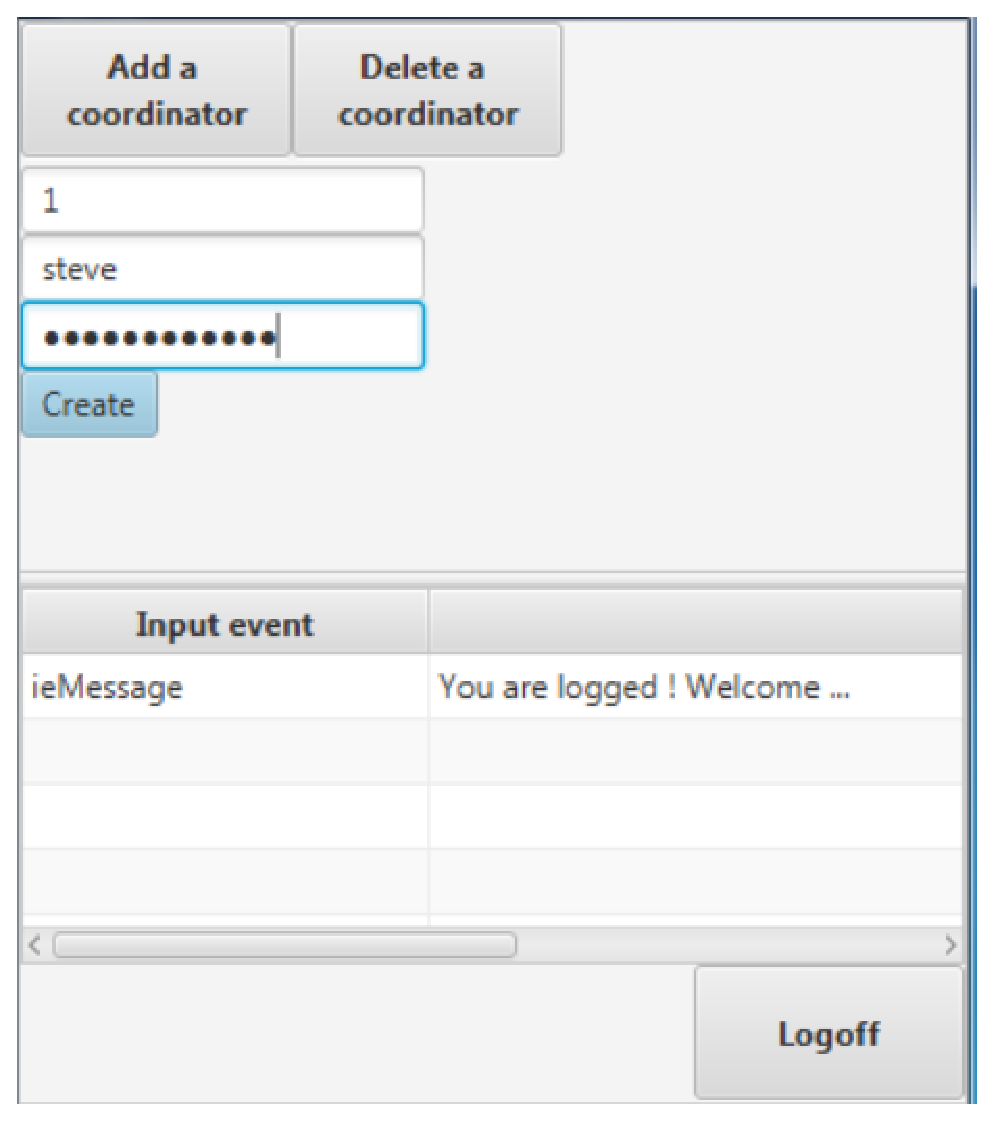
\includegraphics[scale=0.75]{addcoord2.eps}
	\caption{Adding new coordinator}
\end{figure}

\subsubsection{Delete Coordinator}
\vspace{0.5cm}
\hrule
\begin{lyxlist}{PC1}
\small{
\item [\textbf{Procedure:}] DeleteCoordinator
\item [\textbf{Scope:}] Crisis Management System (\emph{CMS})
\item [\textbf{Primary Actor}:] Administrator Kuzme
\item [\textbf{Secondary Actor(s)}:] Coordinator Nikita
\item [\textbf{Goal:}] Delete coordinator Nikita from the system.
\item [\textbf{Level}:] User-Goal level
\item [\textbf{Main~Success~Scenario}]:\\
1. \emph{Kuzma} executes the `login' scenario\\
2. \emph{Kuzma} click button `Delete a coordinator`.\\
3. \emph{Kuzma} enters ID `2`. \\
4. \emph{Kuzma} click button `Delete`. \\
4. \emph{Kuzma} \emph{CMS} informs Kuzma that coordinator Nikita is deleted. 
\item [\textbf{Extensions}]:\\
5.a \emph{CMS} informs \emph{Kuzma} that coordinator with ID '2' doesn't
exist.\\ \hspace*{0.5cm} \textbf{procedure ends}
}
\end{lyxlist}
\hrule
\vspace{0.5cm}

\begin{figure}[h]
    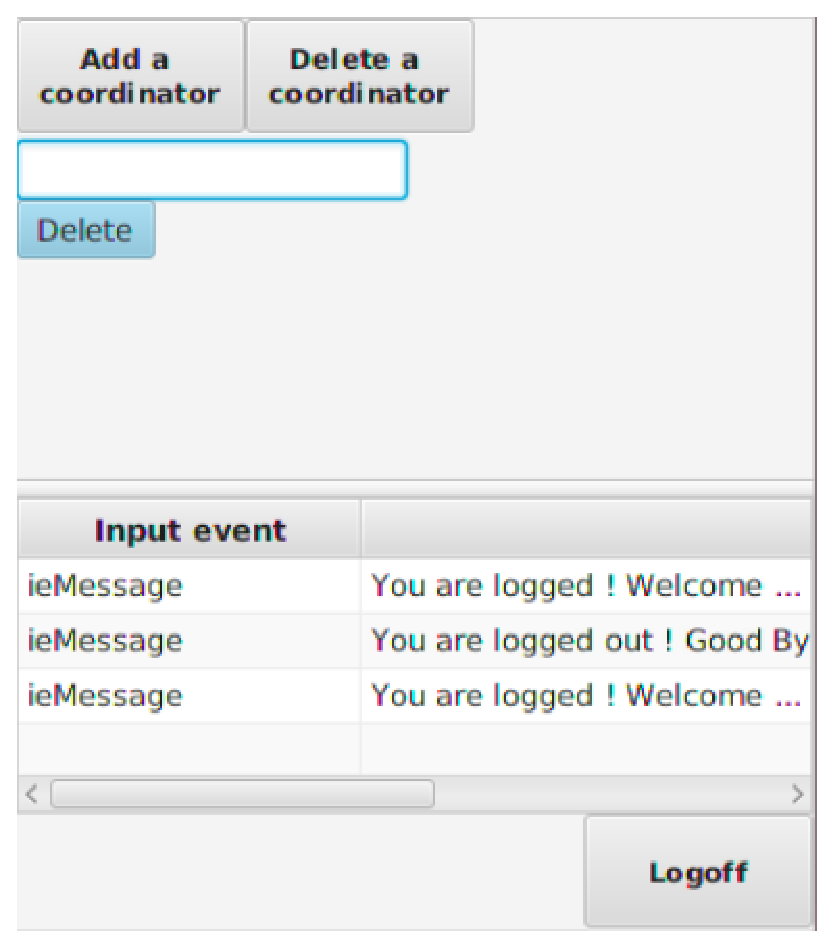
\includegraphics[scale=0.75]{deletecoord.eps}
	\caption{Deleting the coordinator}
\end{figure}


\subsubsection{Get Time Statistics}
\vspace{0.5cm}
\hrule
\begin{lyxlist}{PC1}
\small{
\item [\textbf{Procedure:}] GetTimeStatistic
\item [\textbf{Scope:}] Crisis Management System (\emph{CMS})
\item [\textbf{Primary Actor}:] Administrator Kuzme
\item [\textbf{Goal:}] To get the list of alerts and crises within a defined
period.
\item [\textbf{Level}:] User-Goal level
\item [\textbf{Main~Success~Scenario}]:\\
1. \emph{Kuzma} executes the \emph{login} procedure\\
2. \emph{Kuzma} click button `Statistics`.\\
3. \emph{Kuzma} click on the button "Alerts".\\
4. \emph{Kuzma} click on the radio button `Period of time`.\\
4. \emph{Kuzma} enters '01/28/2017' and '01/29/2017' dates in corresponding text
fields.\\
5. \emph{Kuzma} click button 'Get statistics'. \\
6. \emph{CMS} shows statistics for all the alerts from 01/28/2017 to
01/29/2017.
}
\end{lyxlist}
\hrule
\vspace{0.5cm}

\begin{figure}[h]
    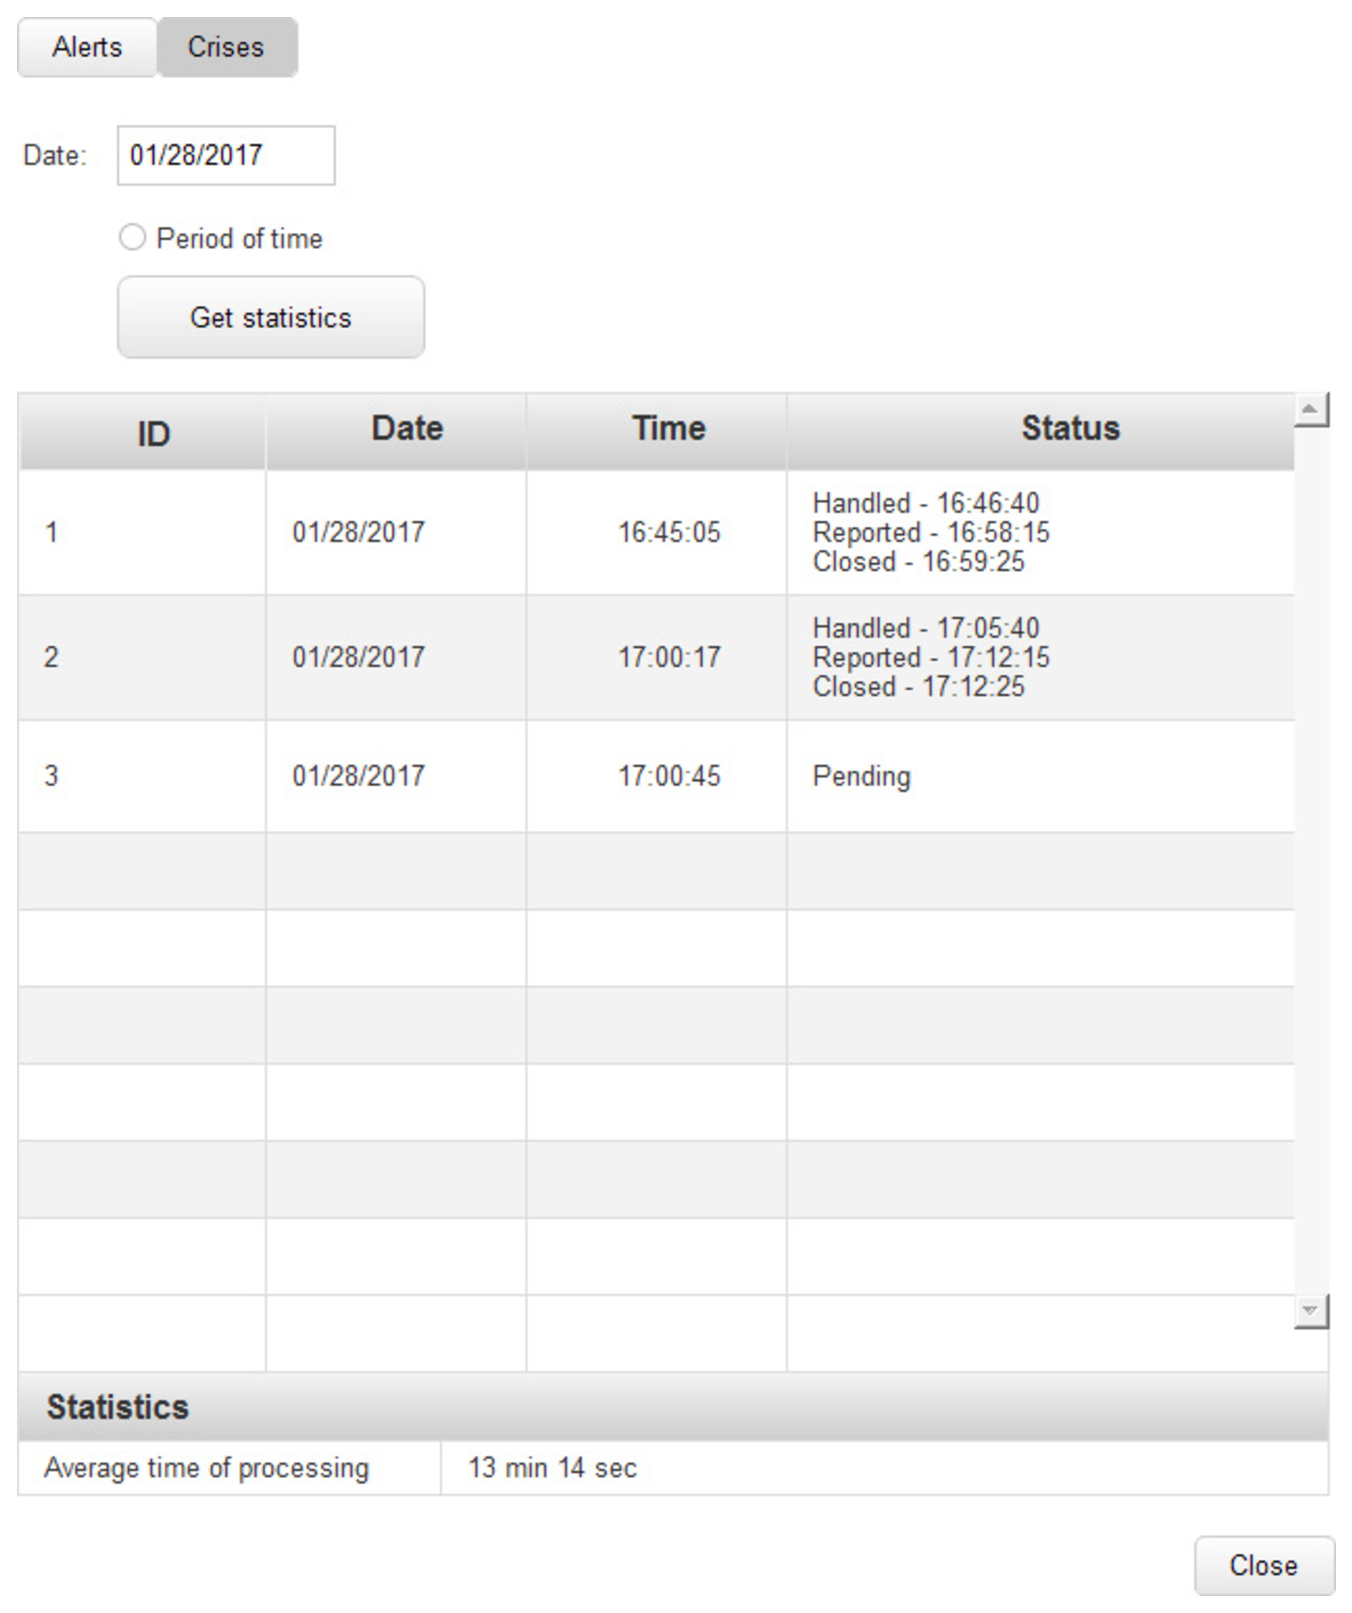
\includegraphics[scale=0.75]{crisis_stats.eps}
	\caption{Get time statistic}
\end{figure}

\subsection{ComCompany}

\subsubsection{Alert creation}
\vspace{0.5cm}
\hrule
\begin{lyxlist}{PC1}
\small{
\item [\textbf{Procedure:}] Alert
\item [\textbf{Scope:}]  Crisis Management System (\emph{CMS})
\item [\textbf{Primary Actor}:] ComCompany ComCom
\item [\textbf{Goal:}] The goal is to create an alert about new car accident and
send it to coordinator.
\item [\textbf{Level}:] User-goal level
\item [\textbf{Main~Success~Scenario}]:\\
1. \emph{ComCom} choose type of the person by clicking on 'victim' row. \\
2. \emph{ComCom} enter current date '2017/02/03'. \\
3. \emph{ComCom} enter contact phone number '+352621854584'. \\
4. \emph{ComCom} enter longitude '4.37274928' and latitude '50.351854584' of a
car crash.\\
5. \emph{ComCom} enter an alert message 'There has been a car crash'.\\
6. \emph{ComCom} set the time '12:43:22' of the alert using scrollbars.\\
7. \emph{ComCom} click the button "Send alert".\\
}
\end{lyxlist}
\hrule
\vspace{0.5cm}

\begin{figure}[h]
    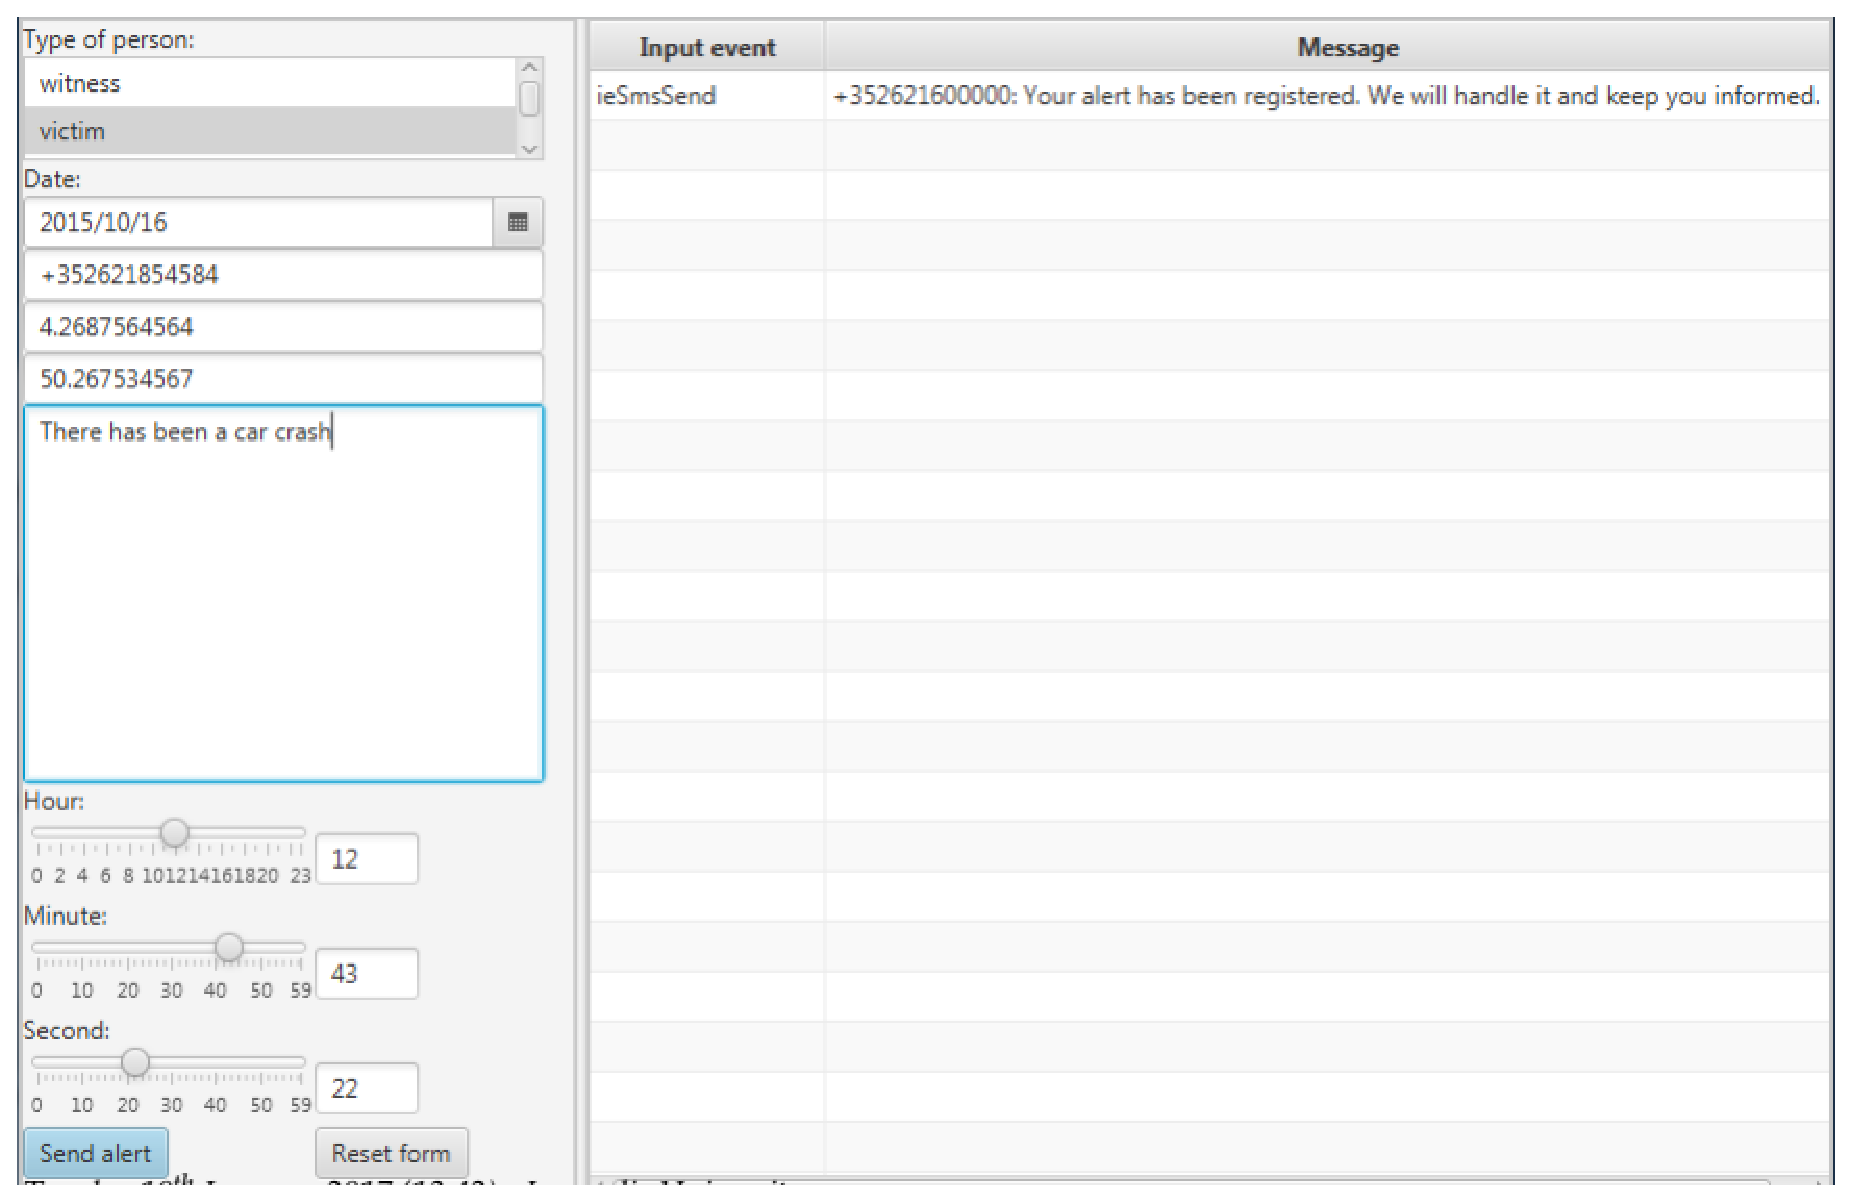
\includegraphics[scale=0.75]{comcom.eps}
	\caption{Alert creation}
\end{figure}

\subsubsection{Information diffusion}
\vspace{0.5cm}
\hrule
\begin{lyxlist}{PC1}
\small{
\item [\textbf{Procedure:}] InformationDiffusion
\item [\textbf{Scope:}]  Crisis Management System (\emph{CMS})
\item [\textbf{Primary Actor}:] ComCompany ComCom
\item [\textbf{Goal:}] The goal is to send information about car crash to
relatives of the victim.
\item [\textbf{Level}:] User-goal level
\item [\textbf{Main~Success~Scenario}]:\\
1. \emph{ComCom} choose type of the person by clicking on 'Family memeber' row.
\\
2. \emph{ComCom} enter current date '2017/02/03'. \\
3. \emph{ComCom} enter contact phone number '+352699954584'. \\
5. \emph{ComCom} enter message 'iCrash Notification System informs you that
Mr.Kuznetsov requires pick-up from car crash location. His coordinates are:
1 Universitetskaya street, Innopolis'.\\
6. \emph{ComCom} set the time '12:43:22' of the alert using scrollbars.\\
7. \emph{ComCom} click the button "Send".\\
}
\end{lyxlist}
\hrule
\vspace{0.5cm}

\begin{figure}[h]
    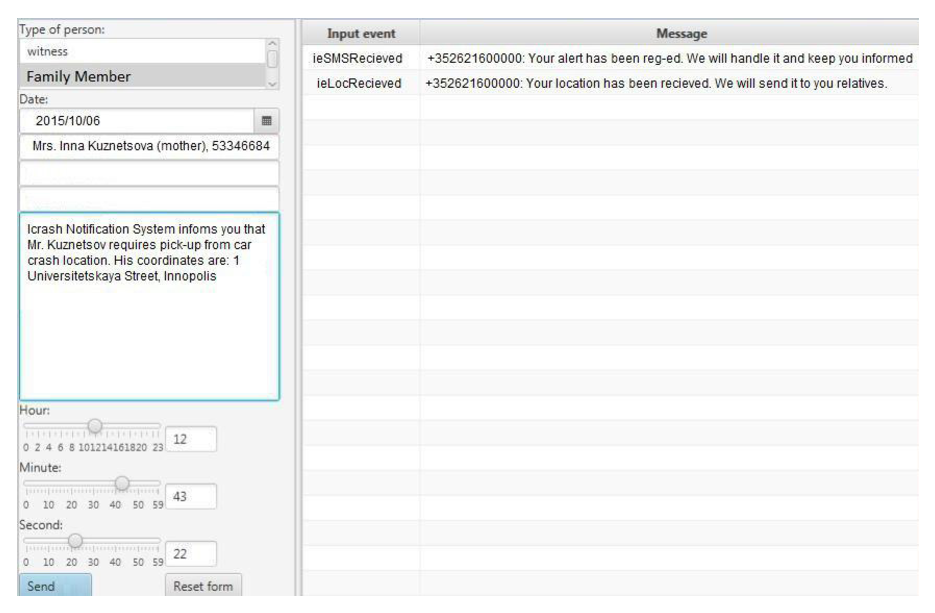
\includegraphics[scale=0.75]{diffusion.eps}
	\caption{Information diffusion}
\end{figure}

\subsection{Coordinator}

\subsubsection{Crisis handling}
\vspace{0.5cm}
\hrule
\begin{lyxlist}{PC1}
\small{
\item [\textbf{Procedure:}] CrisisHandling
\item [\textbf{Scope:}]  Crisis Management System (\emph{CMS})
\item [\textbf{Primary Actor}:] Coordinator Nikita
\item [\textbf{Secondary Actor(s)}:] ComCompany ComCom
\item [\textbf{Goal:}] The goal is to do an action that makes the handling of a
crisis.
\item [\textbf{Level}:] User-goal level
\item [\textbf{Main~Success~Scenario}]:\\
1. \emph{Nikita} executes the \emph{login} scenario. \\
2. \emph{Nikita} gets alert from \emph{ComCom} about new accident. \\
3. \emph{Nikita} press button `Validate` to inform \emph{CMS} that alert with
ID 1 is valid.\\
4. \emph{Nikita} press button `Crises` to open window with current crises.\\
5. \emph{Nikita} select row that contains crisis with ID 1.\\
6. \emph{Nikita} press button `Handle crisis` to inform \emph{CMS} that he
handle this crisis.\\
7. \emph{Nikita} press button `Report on crisis`\\
8. \emph{Nikita} enter a report message '3 have been sent to the hospital' in
report panel.\\
9. \emph{Nikita} press button `Report` in report panel to send report to
\emph{CMS}.\\
10. \emph{Nikita} press button `Close crisis`..\\
}
\end{lyxlist}
\hrule
\vspace{0.5cm}

\begin{figure}[h]
    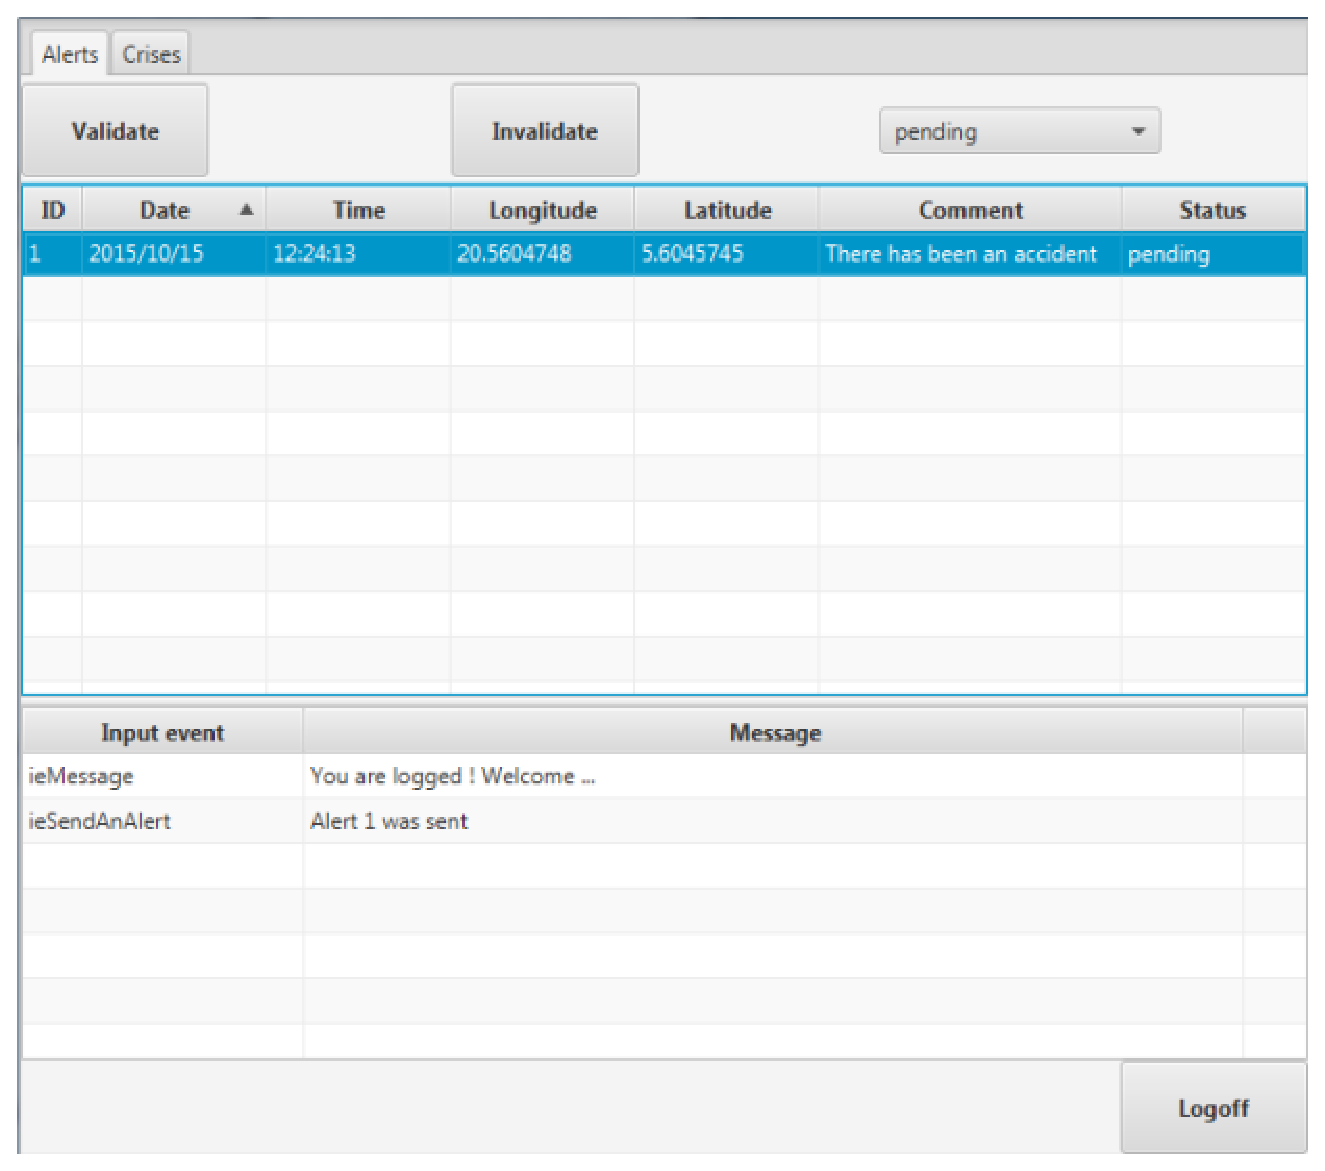
\includegraphics[scale=0.75]{coordinatoralert.eps}
	\caption{Getting new alert}
\end{figure}

\begin{figure}[h]
    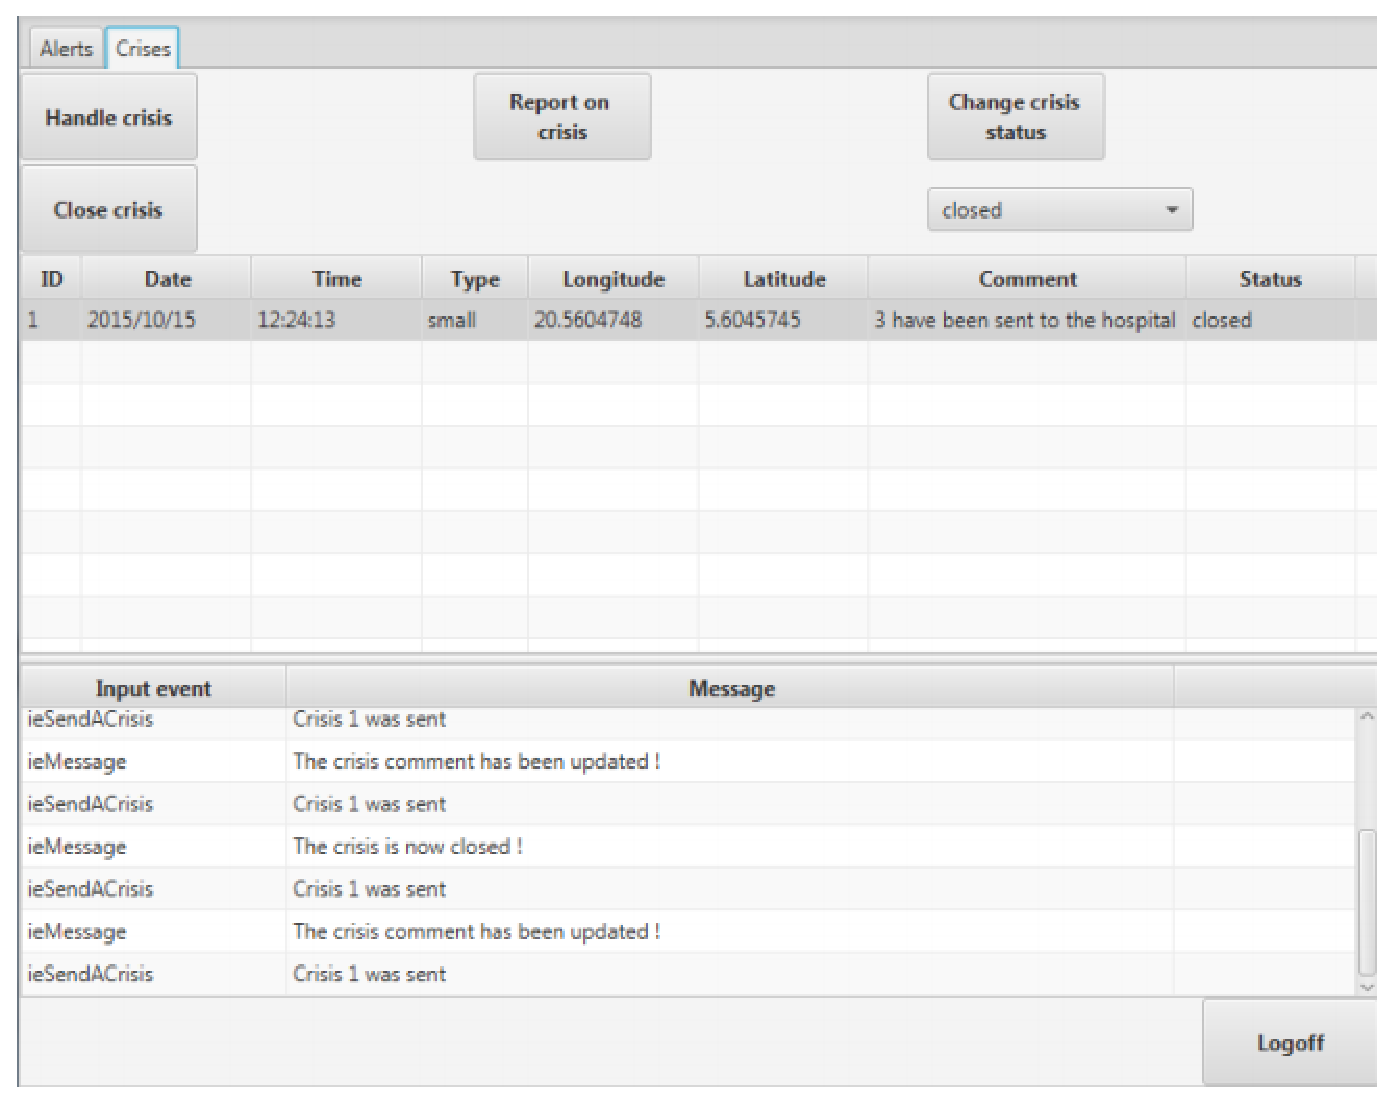
\includegraphics[scale=0.75]{coorinatorcrises.eps}
	\caption{Managing crises}
\end{figure}


\begin{figure}[h]
    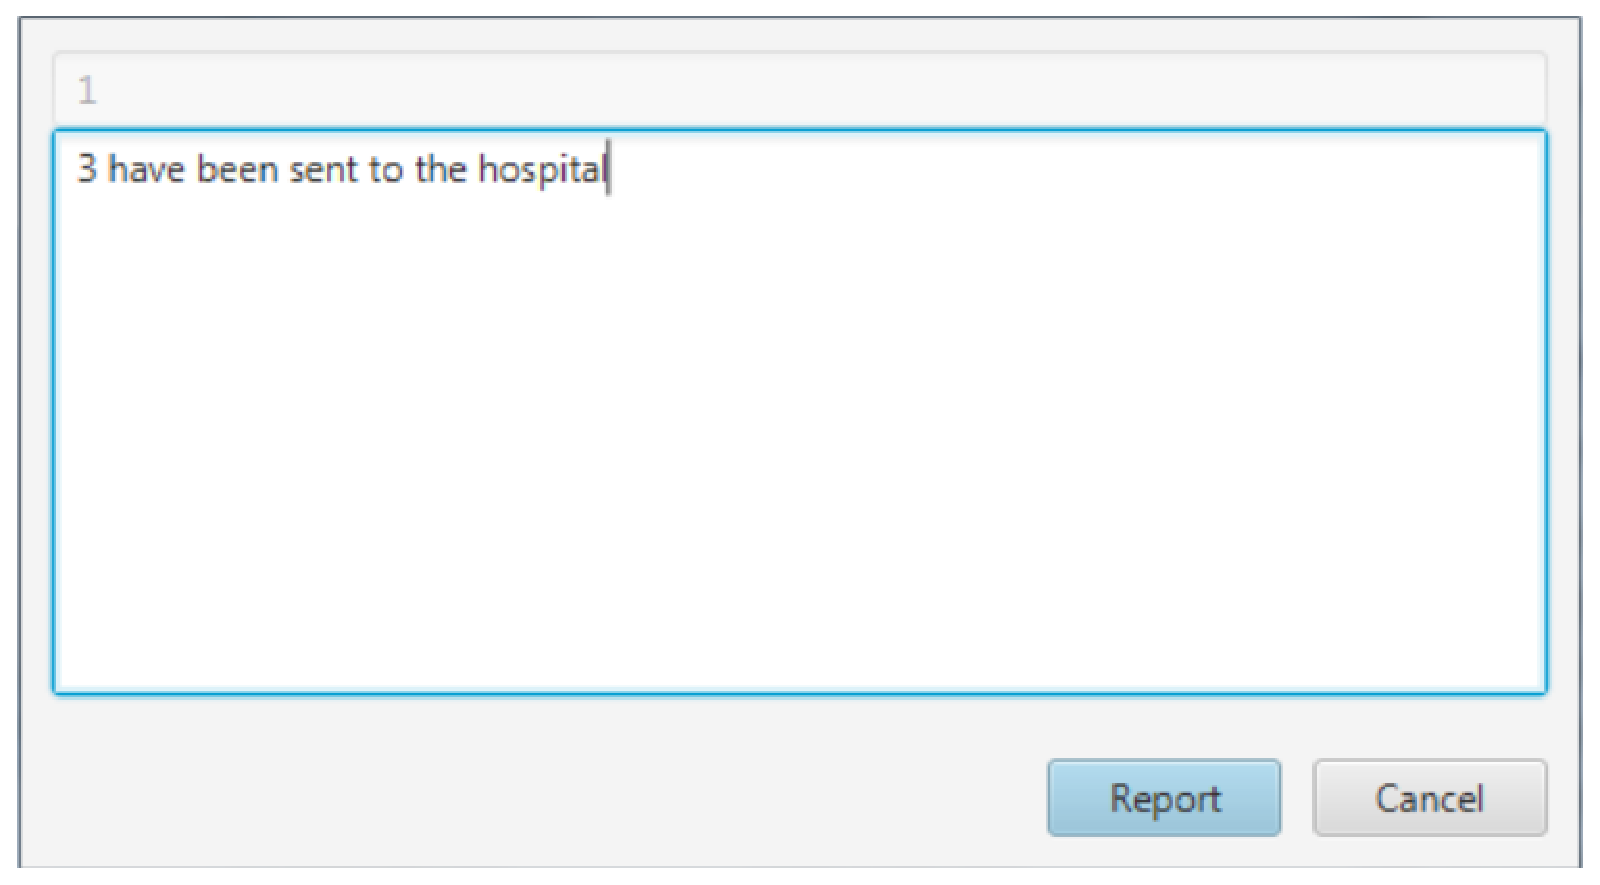
\includegraphics[scale=0.75]{reportpanel.eps}
	\caption{Report panel}
\end{figure}








